\documentclass[12pt, letterpaper]{article}
\usepackage[margin=1.5in]{geometry}    % For margin alignment
\usepackage[english]{babel}
\usepackage[utf8]{inputenc}
\usepackage{algorithm}
\usepackage{graphicx}
\usepackage{float}
\usepackage{amsmath}
\graphicspath{ {./images/} }
% \usepackage{arevmath}     % For math symbols
\usepackage[noend]{algpseudocode}
\title{Poker Agent Literary Review}
\author{Eli Bildman}
\date{3/5/2021}
\begin{document}

\maketitle

In creating an intelligent poker agent of any kind, there are many challenging and unique
problems an engineer must tackle. No limit Texas Hold’em (NLHE) is one of the most recent games to be
effectively played at a high level by a computer. Top poker players were still defeating the best
bots until 2019, when researchers at CMU changed that~\cite{texasholdemaiwin}. This is in contrast to chess masters, who
were defeated in the late 90’s~\cite{chessai}, and Go masters, who famously lost to Google's AlphaGo in
2016~\cite{alphago}. There seems to be something either uniquely human or uniquely nuanced about the
abilities of strong poker players. This review covers the publications of the leading
computer scientists solving these problems, and the strategies they used to create a no limit
Texas Hold’em AI that can efficiently compete with the best poker players today.

Poker is a game of imperfect information. This is in contrast to
games like Chess, Checkers, or Connect Four, games of perfect information~\cite{time-and-space}. In
Poker, players don't have complete information about the state of the game when making their
decisions: what cards other players at the table are holding, as well as what cards will 
be revealed as play progesses. This is what makes poker interesting for humans, but also what makes it challenging for
computers.

The most generic game solving involves creating and traversing a game
tree~\cite{time-and-space}. Game trees are trees where any state of the game is represented by a node. For any node $\beta$,
$\beta$ is connected to parent node $\alpha$ that represents the gamestate one move or random event before $\beta$.
Leaf nodes represent terminal states of the game where no more decisions can be made. These
states have deterministic payoff for all players, called utility. An incomplete game tree for
2-player Poker could look like this:

\begin{figure}[H]
  \centering
  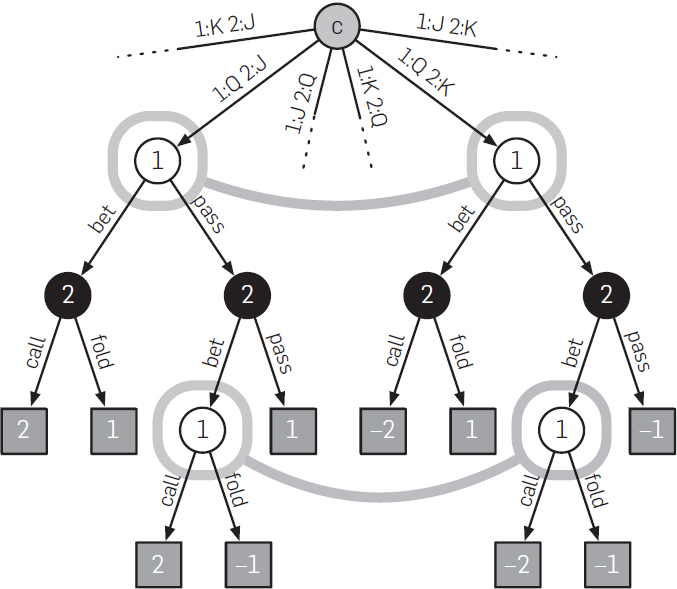
\includegraphics[scale=0.4]{f1}
  \caption{Incomplete Heads-up Poker Gametree~\cite{headsup-limit-solved}}
\end{figure}

\noindent This tree contains a small fraction of the total states possible, but shows how connections are
made between states and their predecessors. The full 2-player poker tree has around $10^{17}$ states~\cite{headsup-limit-solved}.
For simple games, this tree can be fully traversed in a reasonable amount of time.
Meaning a computer could always make the optimal decision based on what choice leads to the
highest utility leaf node. In games of more realistic size, like chess, the game tree is far too large
to be traversed, so this sort of deterministic decision making won’t work. Instead, the tree is
traversed to the extent it can be, then the deepest states found are evaluated based on some evauluation
function, and treated as leaf nodes. For example, in chess, an evaluation function could look at the number
of pieces a player has at a game state and the relative value of those pieces to determine an approximate value. This can also be a good application
for machine learning, as often there are patterns that indicate good game standing that are too complicated
to program by hand. With an accurate enough evaluation function, this strategy can produce
strong decisions.

A similar strategy could be applied to poker, but since some information is unknown to the player when making a decision,
it’s impossible to tell what gamestate is currently at play. Instead, the set of game states with
identical public information, called an ‘information set’ is considered~\cite{cfr-intro}. To similarly solve this
problem with an evaluation function, every possible state of the hidden information on the board has to be considered, and evaluated for.
Including this uncetainty adds another layer of complexity. In poker there are ${52 \choose 2}$, or $1326$ different
combinations cards a player can be dealt. With 2 players, there are ${52 \choose 4}$
or $2.7 \times 10^{5}$ different combinations of dealings.
As in the example earlier, the smallest form of poker has $10^{17}$ states. Even if our evaluation function could reuce this to
$10^{5}$ states and still make usful insights, this leaves us with upwards of $10^{10}$ nodes to explore. In order to reduce the
number of computations needed, more creative algorithms are created.

In order to study these algorithms we define these standard variables and functions for imperfect information games~\cite{cfr-intro}. $A$ is the set of all game actions. $I$ is
an information set, including a number of states that are identical in public information and possible decisions.
$A(I)$ is the set of possible game actions at information set $I$. $T$ and $t$ represent time,
which increments one for each move by a player or random event. A strategy $\sigma^{t}_{i}$ is the set of probabilities that
player $i$ at information set $I_i$ will take any action $a \in A(I_{i})$ at time $t$. All player strategies at time $t$ coalesced 
create strategy profile $\sigma^{t}$. $\sigma_{I\rightarrow a}$ is a strategy profile equivilent to $\sigma$, except
action $a$ is always chosen at $I$.
History $h$ is a sequence of actions and random events starting from the
begining of the game. $\pi^{\sigma}(h)$ is the probability of history $h$ happening with strategy profile $\sigma$.
Similarly, $\pi^{\sigma}(I)$ is the probability of reaching information set $I$ with strategy profile $\sigma$. The counterfactual reach probability of
information set $I$, denoted $\pi^{\sigma}_{-i}(I)$ is the probability of reaching $I$ with strategy
profile $\sigma$ except every decision player $i$ makes is considered to have probability of $1$.
$Z$ denotes the set of terminal game histories. So, if $h \subset z$, $h \neq z$ and $z \in Z$ then h is a nonterminal game history.
$\pi^{\sigma}(h, z)$ represents the probability of terminal history $z$ given non terminal history $h$.
Lastely, $u_{i}(z)$ is defined as the utility, or value recived for player $i$ at terminal history $z$.

The most popular starting algorithm is called “counterfactual regret minimization” or CFR~\cite{cfr-intro}. CFR is the process 
of trying to minimize "regret," which is calculated as a loss of "counterfactual value."
Counterfactual value at a nonterminal history $h$ with strategy profile $\sigma$ is defined as:
\begin{equation}
  v_i(\sigma, h) = \sum_{z \in Z, h \subset z} \pi^{\sigma}_{-i}(h)\pi^{\sigma}(h, z)u_{i}(z)
\end{equation}
This is the counterfactual probability of reaching an endstate, meaning the actions of player $i$ are considered given,
multiplied by the value of that state, summed for every state reachable. This is similar to the expected value of a
gamestate, but done counterfactually. Counterfactual regret builds on this and is defined as:
\begin{equation}
  r(h, a) = v_{i}(\sigma_{I \rightarrow a}, h) - v_{i}(\sigma, h)
\end{equation}
Regret can be considered the difference in value between changing the strategy to choose action $a$ and not.
If this regret is positive, it would be beneficial to change the strategy to make action $a$. Lastly,
counterfactual regret at an infoset $I$ at time $T$ is defined as:
\begin{equation}
  r(I, a) = \sum_{h \in I} r(I, a)
\end{equation}
This needs to be calculated becuase, as discussed earlier, players must consider states in infosets,
and can never know that true history $h$ they're in.

From here, CFR creates a vector of running regret sums for every infoset. Whenever a given infoset is reached, new regrets are calculated and added to these sums. Strategy $\sigma_{i}$ is then updated
to represent the positive regret sums normalized to sum to one. For example, if we had a regret sum vector
$[-5, 10, 8, -2]$, our resulting strategy for $I$ would be $[0, \frac{10}{18}, \frac{8}{18}, 0]$.
This process is repeated an arbitrarily large number of times in a
training process, and it's been shown that~\cite{regret-min-incomplete-information}, if implemented correctly, the strategy profile created
converges to the optimal values.

CFR removes the need to consider every possible state of the unknown variables of a
game because all calculations are done retroactively, when unknown variables are uncovered.
However, CFR still requires calculating the value of every move that could have been
made, which can take too long in large games. To tackle this issue
CFR+ was developed~\cite{cfr-plus}. CFR+ makes the key change of only considering positive regrets when
calculating regret sums. This small difference means the training spends less time rewarding
good decisions, and more time punishing bad ones which, based on studies in the same paper, makes the values
converge faster in most cases.

The last addition to the algorithm is called “Regret Discounting”~\cite{discounted-regret}. It’s notable that for some payout distributions, CFR and CFR+
take exceptionally long to converge due to regrets calculated in early iterations. And example given in “Solving
Imperfect Information Games via Discounted Regret Minimization” is the case of three choices
with payoffs $[0, 1, -1000000]$. In this case, the positive regrets would be
$[333332.5, 333334.5, 0]$. Since the third option has zero regret, it will never be chosen, and
the strategy will consist of picking between options one and two with about $50\%$ odds. The difference
in regret between these choices is very small, so finally converging to the point where
option two is chosen over one will take hundreds of thousands of iterations. The solution to this is to add a weight to the calculation of the
normalized regrets. The normalization step in CFR is really taking the average of the regrets of
every iteration of the training so far. Since the regrets of early iterations are relatively less
important than the regrets found more recently, these regrets can be less heavily weighted. The
weight of a regret iteration is found with the equation $w = max\{T-d, 0\}$. Where $d$ is some
optional delay value to keep early iterations from being affected.

Overall, there're many approaches to solving the unique problems poker and other games
of imperfect information present. These approaches tend to revolve around CFR and therefore,
CFR and the additions that have been made to it will be my main design strategy in creating my
no-limit Texas Hold’em agent.

\bibliographystyle{plain}
\bibliography{bibby}

\end{document}
